\documentclass[journal]{IEEEtran}
\usepackage{amsmath,amssymb,amsthm}
\usepackage{graphicx}
\usepackage{booktabs}
\usepackage{cite}
\usepackage{url}
\usepackage{xcolor}
\usepackage{microtype}
\usepackage{pgfplots}
\pgfplotsset{compat=1.16}

\newtheorem{proposition}{Proposition}
\newtheorem{theorem}{Theorem}
\newtheorem{lemma}{Lemma}
\newcommand{\ours}{FORTRESS-FL}

\begin{document}

\title{Certified Federated Unlearning for IoT: Ledger-Anchored Revocation with Anytime-Valid Forgetting Certificates}

\author{Quang-Vinh Dang%
\thanks{Q.-V. Dang is with British University Vietnam, Hung Yen, Vietnam. E-mail: vinh.dq4@buv.edu.vn.}%
}

\maketitle

\begin{abstract}
Federated learning lets IoT devices train a shared model without exporting data, but a device's influence stays in the model after it leaves, and regulation, decommissioning and poisoned contributions all demand removal. We add an unlearning and governance layer to the FORTRESS-FL robust aggregation system: a hash-chained ledger anchored at independent witnesses, per-round checkpoints of model and reputation state, a consent registry, and Ed25519-signed forgetting certificates. Clients plant paired ghost canaries before training, and an anytime-valid e-process verifier (VOUCH) certifies a revocation wave without retrained references or backdoor markers. We contribute incremental certified recovery (ICR), which audits after each block of recovery rounds under a union-bound error budget and never uses more client rounds than retraining, entanglement-targeted recovery driven by the ledger, a power check that reports when the audit cannot see leakage, a strict reveal rule against selective disclosure, and a deadline-aware wave scheduler. On a synthetic fleet, smartphone sensor data (UCI HAR) and botnet traffic from nine real IoT devices (N-BaIoT), with a linear model and an MLP, exactly retrained models were wrongly flagged in 4 of 280 runs under a seeded reveal order and 1 of 180 under a random one (below the 5\% level). Against retraining for a fixed 60 rounds, ICR used 56--97\% less client energy including canary reveal, but against retraining that stops early it was cheaper only on N-BaIoT with the MLP and more expensive on the other settings; targeted ICR was cheaper than early-stopped retraining in four of five settings. An un-unlearned model passed the audit after an operator filtered canaries in 2 of 10 runs, and after a sign-balanced selective reveal in 19 of 20 runs, which the strict reveal rule cut to 1 of 20. The audit has little power for small models, and the certificate bounds canary memorisation, not parameter erasure.
\end{abstract}

\begin{IEEEkeywords}
Federated unlearning, model governance, provenance, anytime-valid inference, Byzantine robustness, Internet of Things.
\end{IEEEkeywords}

\section{Introduction}
\IEEEPARstart{F}{ederated} learning lets IoT devices train a shared model without exporting raw data~\cite{mcmahan2017}, but a device's data keeps influencing the global model long after the device has left. Data protection law gives owners a right to erasure~\cite{gdpr}, devices are decommissioned or change owner, and poisoned contributions are discovered after the fact. Retraining from scratch for every request costs the whole fleet its original training energy and radio traffic, which is not realistic at IoT scale.

Federated unlearning removes a client's influence without full retraining~\cite{liu2021federaser,halimi2022,wu2022kd,liu2024survey,romandini2024}. Two problems remain for deployment. First, the operator has to \emph{show} that the influence is gone. Cryptographic proofs of unlearning exist for centralised models~\cite{eisenhofer2025}; in federated settings, existing checks mark the leaving client's data with backdoor-style markers~\cite{gao2024verifi}, use fingerprints~\cite{goswami2026} (whose paper gives no test or error bound), or log unlearning requests and actions on a blockchain~\cite{zuo2024}, while BlockFUL addresses how to unlearn on linked chains and not how to test the result~\cite{blockful2024}; a recent conceptual framework paper sets out entities, goals and metrics for verifiable federated unlearning~\cite{nguyen2026}. Second, verification is almost never tied to cost: an operator who must pay for a certificate has little reason to choose a cheap method unless the certificate tells them whether it was enough, and the honest comparison is with retraining that stops when the model has converged, not with a fixed number of rounds.

We address both problems in one system built on the \ours{} robust aggregation pipeline~\cite{dang2026fortress} and on the paired-canary verifier VOUCH~\cite{dang2026vouch}. Our contributions are:
\begin{enumerate}
\item \textbf{Ledger-anchored revocation.} A hash-chained provenance ledger with Merkle roots over client updates, a consent registry, and per-round checkpoints of the model \emph{and} of the reputation state. The chain head is published to independent witnesses and certificates are signed with Ed25519, so an operator that rewrites and re-links its own chain is caught.
\item \textbf{Federated paired-canary certificates.} Clients plant paired ghost canaries before training and commit to them in the ledger; after a revocation wave an anytime-valid e-process verifier~\cite{dang2026vouch} issues or withholds an $(\epsilon,\alpha)$ certificate without retrained references or backdoor markers. A strict reveal rule scores unopened pairs as extreme, so selective disclosure cannot buy a certificate.
\item \textbf{Incremental certified recovery (ICR).} Recovery runs on one model in blocks and is audited after each block at level $\alpha/(k(k{+}1))$ (Theorem~\ref{thm:icr}); it never uses more client rounds than retraining. \textbf{Entanglement-targeted recovery} restricts recovery to the retained clients whose logged updates align most with the revoked ones.
\item \textbf{Audit design and limits.} A power check and canary calibration that report when the audit cannot see leakage, a real-record twin audit as an average-case complement, and a deadline-aware wave scheduler.
\item \textbf{Evaluation.} Client energy including canary reveal, per-device and server cost, on a synthetic fleet, UCI HAR~\cite{anguita2013} and N-BaIoT~\cite{meidan2018}, with a linear model and an MLP, against fixed-length and early-stopped retraining, a certified ladder, sharding, a marker verifier and a membership test; an independent forgetting criterion; dropout, asynchrony and staggered enrolment; and attacks on the audit and the ledger.
\end{enumerate}

\subsection*{What is new relative to \ours{} and VOUCH}
This paper builds on two earlier works by the same author, and we state precisely what it adds.
\emph{\ours{}}~\cite{dang2026fortress} is a training-time system: Pedersen-committed updates, spectral Byzantine detection, reputation-weighted aggregation and Gaussian noise. It has no notion of removing a client after training, keeps no per-round state, and offers no audit. \emph{VOUCH}~\cite{dang2026vouch} is a verifier for centralised (language-model) unlearning: it assumes a single trained model and a forget set, and certifies it with paired canaries and e-processes. It has no federated protocol, no client revocation, no unlearning operators, and no cost model.
Table~\ref{tab:delta} lists what each contributes and what is added here. The new elements are: (i) checkpointing of model \emph{and} reputation state, the ledger, the consent registry and the unlearning operators on top of \ours{}; (ii) a federated canary protocol in which clients hold and commit their own pairs and certificates are issued per revocation wave under partial participation; (iii) incremental certified recovery, entanglement-targeted recovery and the verify-then-escalate ladder, with their error accounting (Theorems~\ref{thm:esc} and~\ref{thm:icr}); (iv) the real-record twin audit, the power check and canary calibration, and the wave scheduler; (v) the energy and traffic model; and (vi) experiments on three data sets, two models, and baselines. The e-process verifier and its coverage theorem are used unchanged from VOUCH and are not claimed as new.

\begin{table}[t]
\centering
\caption{Contribution of each work.}\label{tab:delta}
\footnotesize
\begin{tabular}{@{}p{1.9cm}p{1.9cm}p{1.9cm}p{1.9cm}@{}}
\toprule
 & \ours{}~\cite{dang2026fortress} & VOUCH~\cite{dang2026vouch} & This paper \\
\midrule
Setting & federated training & centralised LMs & federated, IoT \\
Byzantine robust & yes & n/a & inherited, tested during unlearning \\
Client removal & no & forget-set only & client waves, operators \\
Per-round state & no & no & model, reputation, updates \\
Provenance & commitments & manifest hash & ledger, Merkle, consent \\
Verification & none & e-process certificate & certificate per wave, ledger-bound \\
Cost-aware choice & no & no & ICR, ladder, scheduler \\
Energy/traffic & no & GPU passes & client model \\
\bottomrule
\end{tabular}
\end{table}

\section{Related Work}
\textbf{Federated unlearning.} FedEraser rebuilds the model from stored historical updates with calibration~\cite{liu2021federaser}; other methods use knowledge distillation~\cite{wu2022kd}, local unlearning by the departing client followed by recovery rounds~\cite{halimi2022}, two-server secure-computation unlearning with a bounded gap to retraining~\cite{certified2024} or on-device teachers~\cite{fedquit2024}. FedRecover estimates client updates to recover from poisoning~\cite{cao2023fedrecover}. Machine unlearning was introduced to make systems forget~\cite{cao2015}, and exact approaches isolate data in shards~\cite{bourtoule2021}. FedRecovery subtracts weighted gradient residuals with calibrated noise~\cite{zhang2023fedrecovery}. Surveys~\cite{liu2024survey,romandini2024} review methods, evaluation metrics and open problems. Our operators (subtraction of stored updates, rollback to the last clean checkpoint, replay, sharding) are standard; the contribution is the audit that decides between them and the recovery that is run under it.

\textbf{Verifying unlearning.} Backdoor-marker verification in federated settings~\cite{gao2024verifi} detects removal through the behaviour of the marker, which requires modifying the data and gives no error guarantee. PrivEraserVerify reports fingerprint-based verification and claims that the unlearned model is statistically indistinguishable from a retrained one~\cite{goswami2026}; its text gives no theorem, test or error rate for the check, and no energy analysis. Eisenhofer et al.\ give a cryptographic definition and SNARK-based proofs for centralised models~\cite{eisenhofer2025}, which in our estimate is too costly for constrained devices, and veriFUL proposes a reference framework of verification entities, goals, approaches and metrics as a conceptual paper~\cite{nguyen2026}. Planted canaries and exposure tests come from the memorisation literature~\cite{carlini2019}. Membership inference is the usual statistical probe~\cite{shokri2017,yeom2018}, but a threshold on an attack score is not a calibrated test, and unlearning definitions need to be auditable~\cite{thudi2022}. Certified removal gives guarantees for particular algorithms and convex models~\cite{guo2020}; ours is a property of the released model, whichever algorithm produced it.

\textbf{Provenance and ledgers in FL.} Blockchain-based designs record unlearning requests and actions for traceability~\cite{zuo2024} or restructure chained models so that they can unlearn, with a live and an archive chain~\cite{blockful2024}. We use a lightweight hash chain with Merkle-tree inclusion proofs~\cite{merkle1980,merkle1987} and, unlike a log of requests, couple it to a statistical test of the result.

\textbf{Anytime-valid testing.} E-processes and betting martingales give tests valid under optional stopping~\cite{ramdas2023,ramdas2024}, and splitting an error budget over successive looks is classical alpha spending~\cite{landemets1983}. VOUCH applies them to centralised unlearning with paired canaries~\cite{dang2026vouch}. We reuse its verifier and theorems as a component and cite them rather than restate them; the federated protocol, ladder, ledger and evaluation are new here.

\section{Problem and Threat Model}
$N$ clients, each with a local data set $\mathcal D_c$, train a model $\theta\in\mathbb R^d$ with $T$ rounds of robust aggregation. In round $t$ a subset of clients participates, each independently with probability $p$. A \emph{revocation wave} $\mathcal W$ is a set of clients whose consent is withdrawn (or whose updates are found poisoned). The operator must release a model $\theta_u$ that no longer carries their influence, and produce evidence that a third party can check.

The operator is honest-but-verifiable: it executes the protocol but may take shortcuts to save cost, which is the temptation the audit has to catch, and we test three concrete shortcuts: filtering out records that look like canaries before training, rewriting and re-linking its own ledger, and letting revoking clients open only favourable pairs. A minority of clients may be Byzantine during training. Clients are not trusted to self-report forgetting. What is certified is the \emph{residual advantage} that a declared class of scores can extract from the canary cohort of the wave on the released model; it is not erasure in parameter space, which no behavioural test can establish. Out of scope: collusion between the operator and all witnesses, adversaries that adapt to the detector over many waves, and copies of the data or models outside the ledger.

\section{System}
\subsection{Training and provenance}
Training follows \ours{}: each client commits to its clipped update with a Pedersen commitment~\cite{pedersen1991}, the server verifies openings, clusters updates spectrally to flag a Byzantine group, aggregates the rest with reputation weights, adds Gaussian noise~\cite{dwork2014} and updates reputations, in the Byzantine-robust aggregation setting of~\cite{blanchard2017}. We gate the cluster split: a group is flagged only if its cross-similarity to the rest is lower than the within-group similarity by more than a margin, so IID honest rounds are not split arbitrarily.

After each round the ledger appends a record containing the round index, the participant list, the Merkle root over leaves $H(\text{client}\,\|\,H(\text{update}))$, the aggregation weights, the flagged clients and the hash of the new model. Each record includes the hash of its predecessor. The server also stores the model and the reputation vector of every round (the checkpoint), and, optionally, the clipped updates themselves. A \emph{consent registry} tracks revocations and marks them fulfilled only after a rollback record exists. \emph{Anchoring.} A chain held by the operator can be rewritten and re-linked, so every $a$ records the operator signs the head with Ed25519 and sends it to $k$ independent witnesses, which store it and countersign. A verifier compares the ledger it is shown with the witnesses' heads: a rewrite before the last anchor changes every later hash and disagrees with them. Certificates are signed with Ed25519, so third parties verify with a public key.

\subsection{Unlearning operators and cost model}
For a wave $\mathcal W$ let $k_0$ be the first round in which any member of $\mathcal W$ participated according to the ledger, and $\theta_{k_0-1}$ its checkpoint. The operators are:
\emph{retrain} (restart from $\theta_0$ on the retained clients);
\emph{rollback} (restore $\theta_{k_0-1}$ and the reputations of that round, then re-run rounds $k_0,\dots,T$ without $\mathcal W$);
\emph{subtract} ($\theta_T+\eta\sum_t\sum_{c\in\mathcal W}w_{c,t}\tilde g_{c,t}$ using the stored clipped updates, and zero reputation);
\emph{subtract+$R$} (subtract, then $R$ fresh rounds);
\emph{replay} (re-apply stored updates of the retained clients from the checkpoint, no client computation);
\emph{sharded} (clients split into cohorts, only the cohorts that hold a revoked client are retrained); and \emph{early-stopped retrain} (retrain, but stop at the first block of 5 rounds whose validation accuracy is within 0.5 points of the model before unlearning).
After a rollback the ledger forks off the contaminated checkpoints and stored updates are purged so that the revoked clients' influence does not survive in the server's own records.

\begin{proposition}
If clients participate independently with probability $p$ in each round and enrol at round 0, the first round $k_0$ in which any of $m$ revoked clients participates satisfies $\Pr[k_0>r]=(1-p)^{rm}$, so $\mathbb E[k_0]=1/(1-(1-p)^{m})$ (about $1$ for $m\ge 5$ at $p=0.6$) and rollback saves at most about one round out of $T$.
\end{proposition}
This is an assumption, not a law: if devices enrol over time, $k_0$ is the earliest enrolment of the wave and rollback saves the rounds before it (Section~\ref{sec:dyn}). Batching helps differently: rollback cost does not grow with $|\mathcal W|$, so the cost per revoked client falls as $1/|\mathcal W|$.

\textbf{Cost model.} A client round with $n_c$ records costs $n_c f$ FLOPs ($f=4d$ for the linear model, $6P$ for an MLP with $P$ parameters), uploads $4P+64$ bytes (float32 update and a 512-bit commitment) and downloads $4P$ bytes. Energy is $e_{\text{flop}}\cdot\text{FLOPs}+e_{\text{bit}}\cdot 8\cdot\text{bytes}$ with $e_{\text{flop}}=1$\,nJ and $e_{\text{bit}}=100$\,nJ, assumptions typical of low-power radios and processors, not measurements. The canary reveal ($2m(d{+}1)\cdot4$ bytes per revoked client) is added to every policy that needs a certificate, retraining included. We report fleet energy, the worst single device, and server storage; server computation is not counted except the entanglement score ($3\,d$ FLOPs per stored update).

\subsection{Paired canaries and the certificate}
Before training, each client draws $m$ twin pairs of exchangeable records from a secret seed (Gaussian features with fair random labels, or crossover records that mix two of its own records feature by feature), flips a coin per pair to pick the in-twin, adds only the in-twin to its data, keeps the ghost, and publishes a digest of the manifest in the ledger. After a wave, the verifier requires the whole committed set of the wave: a committed pair that is not opened is scored as an extreme value, so withholding or cherry-picking pairs can only block a certificate. It scores the released model on both twins with a declared class of scores (loss and signed margin; the test is two-sided, so the sign convention does not matter). If $\theta_u$ carries no influence of the in-twins, each sign of the score difference is a fair coin; betting e-processes on these signs yield (i) a confidence sequence for the residual advantage $\Delta$, (ii) an $(\epsilon,\alpha)$ certificate once evidence that $|\Delta|<\epsilon$ is conclusive, and (iii) a revocation alarm~\cite{dang2026vouch}. The reveal order is drawn from a public beacon in a deployment; the main experiments use a fixed seed for reproducibility and Section~\ref{sec:cal} repeats the calibration with an unpredictable order.

\begin{lemma}[when the null holds]\label{lem:null}
Let $\theta_u=A(\mathcal D_{\rm ret},\xi)$, where $\mathcal D_{\rm ret}$ contains no record of any wave pair and $\xi$ collects participation, dropout, staleness, clipping, reputation weighting, spectral filtering, noise and reveal-order randomness, all drawn independently of the coins. Then each pair's twins are exchangeable given $\theta_u$, each sign is a fair coin, and the e-processes are supermartingales.
\end{lemma}
\emph{Scope.} Retraining on the retained clients, early-stopped or not, satisfies the lemma because every step of the pipeline acts on retained clients' updates only. Subtraction and ICR do not: they use stored updates that depend on the coins, so for them only the one-sided coverage (Theorems~\ref{thm:esc} and~\ref{thm:icr}) holds, and it needs no exchangeability. The guarantees bound the probability of releasing a leaky model as \textsc{issued}; the power check, the utility guard and the \textsc{unpowered} label only withhold releases and cannot raise that probability. Each wave has its own budget $\alpha$; claims across waves need the streaming composition of the verifier with independent coins per wave.

\subsection{Verify-then-escalate}
Let rungs $1,\dots,K$ be operators ordered by cost. The policy runs rung $k$ on a scratch copy, tests its output at level $\alpha/K$, and releases the first rung that is certified and keeps validation accuracy within $\delta$ of the pre-unlearning model. If the last rung does not certify, it is released flagged \textsc{uncertified}. Before the first rung the policy audits the model before unlearning; if that audit does not flag it, the canaries were not memorised, a certificate would hold vacuously, and the final status is reported as \textsc{unpowered} instead of \textsc{issued}.

\begin{theorem}\label{thm:esc}
Let $L$ be the set of rungs whose output has realised cohort advantage at least $\epsilon$ in some score of the declared class. The probability that the policy ever releases a rung in $L$ as certified is at most $\alpha$, for any (data-dependent) stopping rule inside each rung's test and any dependence between rungs.
\end{theorem}
\begin{proof}
By the coverage theorem of the verifier~\cite{dang2026vouch}, each rung $k\in L$ is certified with probability at most $\alpha/K$. A union bound over at most $K$ rungs gives $\alpha$. The utility guard only rejects further rungs and cannot increase the probability of releasing a rung in $L$.
\end{proof}


\subsection{Incremental certified recovery and targeting}
The ladder restarts from the checkpoint for every rung, so a failed attempt is paid for in full. ICR removes this: it audits the pre-unlearning model (power check), applies \emph{subtract}, and then repeats: audit the current model at level $\alpha_k=\alpha/(k(k{+}1))$ and release it if certified and within the accuracy guard; otherwise run a block of $B$ recovery rounds on the \emph{same} model and continue, up to $R_{\max}$ rounds.

\begin{theorem}\label{thm:icr}
Let the audits after blocks $k=1,2,\dots$ be run at levels $\alpha_k=\alpha/(k(k{+}1))$. The probability that ICR ever releases as certified a model whose realised cohort advantage is at least $\epsilon$ is at most $\alpha$. With $R_{\max}\le T$ it uses at most $T$ client rounds, the same as retraining.
\end{theorem}
\begin{proof}
Each audit is a valid level-$\alpha_k$ test of its own model~\cite{dang2026vouch}; since $\sum_k\alpha_k=\alpha$, the union bound gives the first claim for any dependence between the successive models. The round bound is the stopping rule.
\end{proof}
Compared with the ladder (levels $\alpha/K$ for $K$ fixed rungs), ICR needs no $K$ in advance and spends most of the budget on early audits, where most waves stop; the rule is simple alpha spending~\cite{landemets1983}.

\emph{Entanglement-targeted recovery.} From the stored updates, the ledger gives the score $e_c=\frac1{|\mathcal T_c|}\sum_{t\in\mathcal T_c}\cos\!\big(g_{c,t},\bar g_{\mathcal W,t}\big)$ of each retained client $c$, where $\bar g_{\mathcal W,t}$ is the mean logged update of the revoked clients in round $t$ and $\mathcal T_c$ the rounds in which both took part. Recovery then uses only the top $q$ fraction of retained clients. This cuts energy roughly in proportion to $q$; because the audit still decides, a targeted model is released only if certified.

\subsection{Audit design: real twins, power and scheduling}
\emph{Real-record twins.} A client pairs a fraction of its own records at random, a coin decides which twin is trained and the other is withheld. The random matching makes the twins exchangeable, so the same test applies and measures advantage on real records instead of planted noise; the price is withheld data.
\emph{Power check and calibration.} Before unlearning, the audit is run on the model that still contains the wave; if it is not flagged, the canaries were not memorised and the final status is \textsc{unpowered}. Calibration picks the smallest canary count $m$ (then feature scale) on a pilot run for which the audit flags the pilot model.
\emph{Wave scheduler.} Requests wait until the queue holds $P^\star$ canary pairs, or until the oldest has waited $D-\delta$ days ($D$ the legal response period, $\delta$ a margin), whichever comes first.

\section{Experiments}
\subsection{Setup}
\textbf{Data.} \emph{Synthetic fleet:} 60 clients, $d=1024$ features (a linear head on frozen embeddings), ten Gaussian latent classes with binary labels and 8\% label noise, Dirichlet($\alpha{=}1$) split, 12 records per client. \emph{UCI HAR}~\cite{anguita2013,reyesortiz2013uci}: 561 smartphone features, one client per subject (30; dynamic versus static activity). \emph{N-BaIoT}~\cite{meidan2018}: 115 traffic statistics from nine commercial IoT devices infected with Mirai and BASHLITE; we split each device into five sites with disjoint random subsets, giving 45 clients (benign versus attack). Real-data clients keep 40 records. Models are logistic regression and a one-hidden-layer MLP (32 tanh units; 18\,049 parameters on HAR, 3\,777 on N-BaIoT). Each client plants $m=6$ canary pairs; $T=60$, $p=0.6$, update clipping at norm 1, no DP noise unless stated; a wave revokes a third of the clients (20, 10 and 15; 120, 60 and 90 pairs); $\epsilon=0.2$, $\alpha=0.05$; ICR block $B=5$, $R_{\max}=60$.

\textbf{Seeds and inference.} The synthetic operator table uses 10 seeds and everything else 5 or more (calibration 40--60). A seed re-draws the records each client keeps, the canaries, participation and initialisation; the five-site split of N-BaIoT is ours. With five runs, 4 of 5 against 5 of 5 is not a significant difference (the 95\% Clopper--Pearson interval for 4 of 5 is 28--99\%), so we report intervals for the headline rates and read counts only as orders of magnitude; the tables in the Supplement give all counts. Hyper-parameters, figures (S1--S9), tables (S1--S18) and commands are there too.

\subsection{Calibration of the audit}\label{sec:cal}
Over 280 exactly retrained models under the seeded reveal order (synthetic 40; HAR and N-BaIoT, linear and MLP, 60 each) the verifier flagged 4 (1.4\%, 95\% CI 0.4--3.6\%), below $\alpha=5\%$; one of 25 early-stopped retrains was flagged. With an unpredictable (OS-entropy) order, 1 of 180 retrained models was flagged (0.6\%, CI 0.01--3.1\%; synthetic, HAR MLP, N-BaIoT MLP). The un-unlearned model was flagged in 160 of 160 seeded runs on the synthetic fleet and HAR (CI 97.7--100\%) and in 120 of 120 random-order runs there, but in only 36 of 60 for the N-BaIoT MLP (CI 47--72\%) and 9 of 60 for its linear model at $T=30$; elsewhere the model had not memorised the canaries and the certificate that follows says little. The policy audits the model before unlearning and reports \textsc{unpowered} instead of \textsc{issued} when it is not flagged (3 of 5 waves for the N-BaIoT linear model). Retrained models were certified in 51 to 60 of 60 random-order runs, the rest undetermined: the test is conservative, so low false alarms come with limited power.

\subsection{Recovery policies against fixed and early-stopped retraining}\label{sec:icr}
A fixed-length retrain over-provisions when the task converges early, so we add early-stopped retraining (Section~IV-B) as a baseline. Table~\ref{tab:icr} and Fig.~\ref{fig:new} give client energy including canary reveal. Against the fixed 60 rounds, ICR used 66, 56, 78, 68 and 97\% less energy (synthetic, HAR linear, HAR MLP, N-BaIoT linear, N-BaIoT MLP), and these savings changed by at most 3 points over a 100-fold grid of $e_{\rm flop}$ (0.1--10~nJ) and $e_{\rm bit}$ (10--1000~nJ/bit). Against early-stopped retraining, which needed 5, 16, 5, 17 and 8 rounds, plain ICR was \emph{more} expensive on the synthetic fleet and HAR (by 122, 37 and 152\%) and equal on the N-BaIoT linear model, and cheaper only on the N-BaIoT MLP (74\%); the signs did not change over the grid. Targeted ICR ($q=0.25$ of the retained clients) was cheaper than early-stopped retraining by 41, 29, 66 and 92\% on HAR and N-BaIoT but 15\% dearer on the synthetic fleet, and certified one wave less on the synthetic fleet and on HAR with the linear model. ICR's worst run never cost more than retraining by more than 1\%, while the ladder's did in four settings (e.g.\ 119.6~J against 88.1~J on the HAR MLP). The worst single device spent 0.10, 0.12, 3.1, 0.013 and 0.13~J under ICR against 0.30, 0.16, 5.0, 0.035 and 1.1~J under fixed retraining and 0.03, 0.05, 0.58, 0.012 and 0.18~J under early stopping. The server keeps 1.5--155~MB of stored updates, which these figures do not include. The N-BaIoT linear row is unpowered. In short, the benefit of ICR over a sensible baseline is real only where subtraction plus a few rounds beats retraining to convergence, and targeting is what makes it competitive more often.

\begin{table}[t]
\centering
\caption{Mean client energy in J (with canary reveal) / waves certified of 5. N-BaIoT linear: unpowered audit. ``Early'': early-stopped retraining.}\label{tab:icr}
\footnotesize
\setlength{\tabcolsep}{3pt}
\begin{tabular}{@{}lccccc@{}}
\toprule
 & Synth. & HAR & HAR & N-BaIoT & N-BaIoT\\
 & lin. & lin. & MLP & lin. & MLP\\
\midrule
retrain (60 rounds) & 10.4/5 & 2.9/3 & 86.7/4 & 0.95/4 & 27.4/5\\
retrain early & 1.6/5 & 0.94/4 & 7.4/4 & 0.31/5 & 3.6/5\\
ladder & 7.5/5 & 2.0/3 & 25.8/4 & 0.42/1 & 0.95/5\\
ICR & 3.5/5 & 1.3/4 & 18.8/4 & 0.31/1 & 0.95/5\\
ICR $q$=0.25 & 1.8/4 & 0.55/3 & 5.3/4 & 0.11/1 & 0.30/5\\
\bottomrule
\end{tabular}
\end{table}

\begin{figure*}[t]
\centering
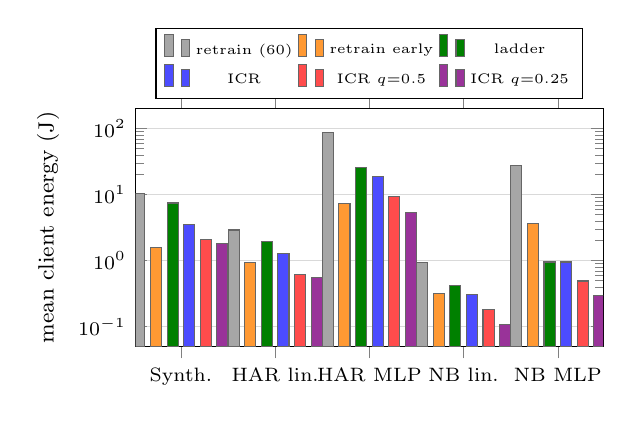
\begin{tikzpicture}
\begin{axis}[ybar,log origin=infty,width=0.62\textwidth,height=4.6cm,ymode=log,ymin=0.05,ymax=200,bar width=4pt,
 symbolic x coords={Synth.,HAR lin.,HAR MLP,NB lin.,NB MLP},xtick=data,x tick label style={font=\scriptsize},
 y tick label style={font=\scriptsize},ylabel={mean client energy (J)},ylabel style={font=\footnotesize},
 legend style={font=\tiny,at={(0.5,1.04)},anchor=south,legend columns=3},enlarge x limits=0.12,ymajorgrids,grid style={gray!30}]
\addplot[fill=gray!70,draw=black!60] coordinates {(Synth.,10.4222) (HAR lin.,2.9071) (HAR MLP,86.6957) (NB lin.,0.9494) (NB MLP,27.4304)};
\addlegendentry{retrain (60)}
\addplot[fill=orange!80,draw=black!60] coordinates {(Synth.,1.5854) (HAR lin.,0.9413) (HAR MLP,7.4486) (NB lin.,0.3139) (NB MLP,3.6344)};
\addlegendentry{retrain early}
\addplot[fill=green!50!black,draw=black!60] coordinates {(Synth.,7.4632) (HAR lin.,1.9587) (HAR MLP,25.7716) (NB lin.,0.4223) (NB MLP,0.9511)};
\addlegendentry{ladder}
\addplot[fill=blue!70,draw=black!60] coordinates {(Synth.,3.5255) (HAR lin.,1.2865) (HAR MLP,18.7558) (NB lin.,0.3066) (NB MLP,0.9511)};
\addlegendentry{ICR}
\addplot[fill=red!70,draw=black!60] coordinates {(Synth.,2.0842) (HAR lin.,0.6142) (HAR MLP,9.2327) (NB lin.,0.1812) (NB MLP,0.4913)};
\addlegendentry{ICR $q{=}0.5$}
\addplot[fill=violet!80,draw=black!60] coordinates {(Synth.,1.8180) (HAR lin.,0.5512) (HAR MLP,5.3029) (NB lin.,0.1069) (NB MLP,0.2993)};
\addlegendentry{ICR $q{=}0.25$}
\end{axis}
\end{tikzpicture}\hfill
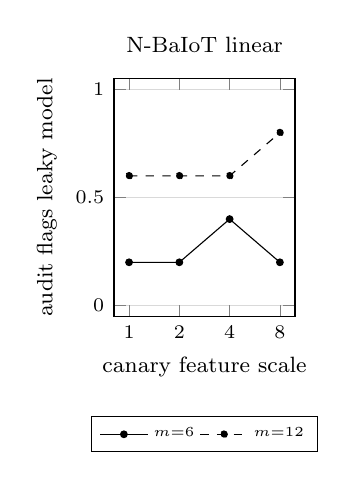
\begin{tikzpicture}
\begin{axis}[width=0.32\textwidth,height=4.6cm,xmode=log,log basis x=2,xlabel={canary feature scale},xlabel style={font=\footnotesize},
 ylabel={audit flags leaky model},ylabel style={font=\footnotesize},ymin=-0.05,ymax=1.05,xtick={1,2,4,8},xticklabels={1,2,4,8},
 x tick label style={font=\scriptsize},y tick label style={font=\scriptsize},legend style={font=\tiny,at={(0.5,-0.42)},anchor=north,legend columns=2},ymajorgrids,grid style={gray!30},title={\footnotesize N-BaIoT linear}]
\addplot[solid,mark=*,mark size=1.2pt] coordinates {(1,0.20) (2,0.20) (4,0.40) (8,0.20)};
\addlegendentry{$m{=}6$}
\addplot[dashed,mark=*,mark size=1.2pt] coordinates {(1,0.60) (2,0.60) (4,0.60) (8,0.80)};
\addlegendentry{$m{=}12$}
\end{axis}
\end{tikzpicture}
\caption{Left: mean client energy per recovery policy including the canary reveal (log scale; 5 seeds). Right: share of runs in which the audit flags the un-unlearned N-BaIoT linear model, against the canary feature scale for $m=6$ and $m=12$ pairs per client.}\label{fig:new}
\end{figure*}

\subsection{Does a certificate track forgetting?}
The canary test is its own ground truth, so we check it against criteria it does not use: the parameter distance to a retrained model, normalised by the distance between two independent retrainings (the retraining noise floor), the prediction disagreement with the retrained model, and the loss on the revoked clients' real records relative to the retrained model (1.0 means the same). The un-unlearned model has loss ratios of 0.18 (synthetic), 0.05 (HAR) and 0.87 (N-BaIoT) and is flagged in the first two; among the certified runs of subtraction, ICR and recovery the median ratio is 1.9, 1.06 and 1.7 and the smallest is 1.29, 0.91 and 1.0. So certified models fit the revoked clients' real records about as badly as a retrained one or worse (smallest ratio 0.91), and flagged ones fit them much better. Certification does not imply parameter equivalence: certified operators sit 1.5--4.6 noise floors from the retrained parameters, the un-unlearned model 2.4--8.1, so operators close about half of the gap. Prediction disagreement with retraining was at most 4\% for every operator except plain subtraction (37\% on the synthetic fleet, 3.5--14\% on N-BaIoT). The independent criterion has little discriminating power on N-BaIoT (0.87 for the un-unlearned model), consistent with the weak audit there.

\subsection{Operators, waves and heterogeneity}
On the synthetic fleet (10 seeds) the un-unlearned model is flagged in 10 of 10 runs. Plain subtraction and replay cost no client energy but cost accuracy (0.62), which the certificate cannot see: it was issued in 4 of 10 runs, so every policy carries an accuracy guard. Subtraction followed by 5, 10 and 20 recovery rounds restores accuracy (0.98) and is certified in 4, 4 and 6 of 10 runs at 0.8, 1.6 and 3.2~J, against 8 of 10 for retraining at 9.6~J; no operator is certified every time because 120 pairs is near the test's resolution at $\epsilon=0.2$. Rollback restored round 0 in every run (Proposition~1). The ladder of Section~IV-C certified 10 of 10 waves against 8 of 10 for retraining, but this is partly noise: in two seeds retraining was undetermined while the ladder released an approximate model, and the ladder is tested at $\alpha/4$ over up to four attempts. Its cost is bimodal (0.8 to 13.8~J, mean 6.6~J against 9.6~J), which ICR replaces. Retraining cost per revoked client falls from 3.4~J for waves of 4 to 0.24~J for waves of 30; serving 20 requests singly is a model estimate (14.0~J each, extrapolated from three requests). Poisoned clients (3 or 8, half their data stamped with a trigger) gave a backdoor success rate of 0.29 and 0.71, reduced to 0.007 and 0.002 by subtraction plus 10 rounds, against 0.027 for retraining and 0.029 for a clean model, at 2.1--2.3~J against 12.5--13.8~J; this held with 12 Byzantine clients present. Operators were certified more often with stronger heterogeneity, lower participation and more DP noise; we did not isolate the cause. At $d=64$ the un-unlearned model was certified in 3 of 5 runs, since it cannot memorise the canaries (Supplement S1, S2, Figs.~S1--S4).

\subsection{Real IoT data}
On HAR and N-BaIoT (Supplement Table~S3, Figs.~S5--S9) the un-unlearned MLP was flagged in 5 of 5 runs on both, the HAR linear model in 5 of 5 and the N-BaIoT linear model in 1 of 5, so its certificates are vacuous. Cheap operators were certified about as often as retraining for the MLP; on N-BaIoT plain subtraction cost accuracy for the linear model (0.871 against 0.995). A trigger on 2 or 5 N-BaIoT clients implanted (success 0.25 and 0.45 linear, 0.36 and 0.59 MLP) and subtraction with 10 rounds reduced it to 0.003--0.010 at 0.2~J instead of 1.3~J (linear) and 6.6~J instead of 39.3~J (MLP); on HAR no trigger implanted (at most 7\%), so HAR says nothing about poisoning. A single client could be certified on the HAR MLP with $m=60$ (flagged 5 of 5, retrained certified 5 of 5, subtract+20 4 of 5) at the price of canaries being 60\% of its records; on N-BaIoT the audit had no power at this size (flagged 0 of 5 at $m=60$, 2 of 5 with 128 hidden units and $m=100$).

\subsection{Dropout, asynchrony, enrolment, sharding and request granularity}\label{sec:dyn}
\textbf{Dynamics.} With 30\% dropout of selected clients, gradients computed on models up to 3 rounds old, both, and staggered enrolment (devices join over the first 40 rounds), ICR used 8--40\% of the energy of retraining in all 15 setting-variant cells, with certification counts equal to the base case apart from one extra wave. Under simultaneous enrolment rollback equals retraining; under staggered enrolment the wave's earliest participation was round 27 on average, rollback restarted from round 26 and saved 44\% of retraining energy, still above ICR (Table~S13).
\textbf{Sharding.} With four cohorts, a wave inside one cohort cost 18--20\% of monolithic retraining (2.4 against 13.3~J synthetic; 0.68 against 3.4~J HAR linear; 21.7 against 108.8~J HAR MLP), a wave spread over all cohorts 1.0--1.14 times it, and ensemble accuracy was equal on HAR (0.999) and higher on the synthetic fleet (1.00 against 0.983). A one-cohort wave has too few pairs for a certificate (2--4 of 5 issued). \textbf{Granularity.} Removing the mirai\_udp attack family on N-BaIoT left accuracy on it at 0.986 (linear) and 1.000 (MLP) after retraining against 1.000 before, since the detector generalises; removing 25\% of the largest client's records moved parameters by 0.95--1.12 noise floors after retraining against 0.85--1.16 before. Both are below the retraining noise, so neither request has a measurable effect at this scale, and rollback again equals retraining.

\subsection{Attacks on the audit and the ledger}
\textbf{Filtering canaries.} An isolation forest separates Gaussian canaries from real records with AUC 0.94 (HAR) and 0.92 (N-BaIoT) and crossover canaries with 0.70 and 0.71. An operator that drops as many top-scoring records as there are canaries removes 59 and 48\% of Gaussian canaries and 34 and 28\% of crossover ones. The model it then trains on the rest, never unlearned, was certified in 2 of 10 runs with Gaussian canaries and 7 of 10 with crossover canaries; but crossover canaries have little power (the honest un-unlearned model was flagged in 3 of 10 runs against 10 of 10), so stealth costs sensitivity. \textbf{Selective reveal.} If revoking clients open a sign-balanced subset of their pairs and the verifier accepts partial reveals, the un-unlearned model was certified in 19 of 20 runs; with the strict rule (unopened pairs scored as extreme) in 1 of 20. \textbf{Ledger.} Re-linking a rewritten record leaves the chain valid (detected in 0 of 300 trials); with three witnesses anchored every 5, 10, 20 and 60 records, 92, 89, 73 and 2\% of 300 random rewrites were caught (those after the last anchor escape), and receipts cost 7.8~kB at the shortest interval. Ed25519 signatures verified in 200 of 200 cases and 200 of 200 status edits were detected. The ledger holds 61 records for 60 rounds and 101~kB (about 1.1\% of upload traffic); checking the chain takes 1.6~ms and a Merkle proof 5~$\mu$s. After unlearning, checkpoints take 17--703~kB and stored updates 11.5--21.8~MB.

\subsection{Real-record twins, canary calibration, scheduler and baselines}
With real twins (about 100 pairs on HAR and 150 on N-BaIoT) the advantage bound was 0.17--0.23 for the un-unlearned model and every operator, so the real-record audit certified each of them in 4 or 5 of 5 runs (one N-BaIoT MLP run was flagged for the un-unlearned model, the retrained one and two operators alike, the false-alarm level); over 50 more seeds it flagged the un-unlearned HAR and N-BaIoT MLPs in 1 and 3 runs and the retrained ones in 1 and 2, the false-alarm level. These models leak no real-record advantage above $\epsilon=0.2$ even without unlearning, and the canary audit is the sensitive probe. On the N-BaIoT linear model, doubling $m$ helped more than scale (flagged 1--2 of 5 at $m=6$, 3--4 of 5 at $m=12$), and neither made the audit reliable. A simulated year of Poisson revocations ($D=30$ days, $m=6$, power target 120 pairs, wave energy 2.7~J from the synthetic ICR run) gave 12-fold less energy per request than serving each request at once at 1 request per day (mean latency 10.3 days, 7\% underpowered waves), and at 0.2 per day every batched wave hit the deadline underpowered. A marker verifier in the style of VeriFi~\cite{gao2024verifi} and a loss-threshold membership test~\cite{yeom2018}, as we implemented them and without tuning, did not separate the un-unlearned from the retrained model on HAR and N-BaIoT (marker success 0.034 against 0.034 and 0.40 against 0.43; AUC 0.44 against 0.44 and 0.43 against 0.42), where the canary audit flagged the former in 10 of 10 runs and certified the latter in 9 of 10. Since these models leak no real-record signal, the result shows that a fixed trigger or threshold needs calibration that the e-process does not, not that those methods fail where leakage exists.

\section{Discussion and Limitations}
\label{sec:disc}
\textbf{What a certificate means.} It bounds the advantage that two declared scores extract from the canary cohort of the wave on the released model, at any stopping time, and the guarantee covers \textsc{issued} releases only (Lemma~\ref{lem:null} and Theorems~\ref{thm:esc}, \ref{thm:icr}). It is not erasure in parameter space: certified operators stayed 1.5--4.6 retraining-noise floors from the retrained parameters. It tests canary memorisation; the models here leak no real-record advantage above $\epsilon=0.2$ even without unlearning, so the real-record twin audit cannot discriminate and the canary audit is the sensitive probe, which a cheaper operator can pass while leaving subtler influence on real records. The statement is therefore ``the canary-extractable advantage is below $\epsilon$'', not ``the data are forgotten''. The ledger audit certifies lineage only.

\textbf{Where the contribution is thin.} The e-process verifier and its coverage theorem come from VOUCH~\cite{dang2026vouch}; Theorems~\ref{thm:esc} and~\ref{thm:icr} are union bounds over it, Lemma~\ref{lem:null} only spells out when its null applies, and the operators are standard. The new content is the federated protocol and its hardening, the recovery policies, the cost accounting and the evaluation. The honest comparison also weakens the headline: against retraining that stops early, plain ICR is not cheaper on three of five settings, and its advantage depends on how fast the task converges.

\textbf{Limits of the evidence.} Three data sets (one synthetic, two real, of which HAR is easy and N-BaIoT is split into sites by us), a linear model and a one-hidden-layer MLP, 5--10 seeds (intervals in the Supplement), simulated clients, a modelled energy cost with fleet totals, worst device and server storage but no measured device energy, and canaries that take up much of a small buffer. The audit's power depends on model capacity: it was weak for the N-BaIoT models, and per-client certificates worked only for the HAR MLP. Several operators are certified as often as retraining, which says the test is blunt at this resolution as well as that the operators work. The attacks we ran are single-shot (a fixed isolation-forest filter, one selective-reveal rule); an operator adapting over many waves, colluding with all witnesses, or hiding copies of the data outside the ledger is out of scope. Anchoring protects only records older than the last anchor. Request-level experiments on class and sample removal found no measurable effect, so they do not exercise the pipeline; feature-level forgetting is not supported, and hierarchical or cross-silo federations are covered only by the cohort-sharded operator.

\textbf{Regulatory alignment.} The ledger and the certificate give a data controller a verifiable record that a revocation was honoured; whether this satisfies a specific legal duty (for example under GDPR Art.~17~\cite{gdpr}, or obligations emerging under the EU AI Act) is a question for counsel, and we make no such claim. Holding requests to reach a wave size, as the scheduler does, must be agreed with the regulator or the data subject; we use 30 days only as an example deadline.

\section{Conclusion}
We built an unlearning and governance layer for federated IoT learning in which the acceptance test is a statistical audit with a stated error budget, the ledger is anchored at independent witnesses and certificates are publicly verifiable. Across a synthetic fleet, smartphone sensor data and botnet traffic from nine IoT devices, the audit wrongly flagged an exactly retrained model in about 1\% of runs and flagged the un-unlearned model whenever the canaries were memorised, and it reported when they were not. Incremental recovery used 56--97\% less client energy than retraining for a fixed 60 rounds but, against early-stopped retraining, helped only where subtraction plus a few rounds beat retraining to convergence, and targeting made it competitive on four of five settings. Selective reveal and canary filtering can defeat a naive audit; a strict reveal rule closed the first, and the second trades sensitivity for stealth. Next steps are deeper networks and more IoT modalities, measured device energy, canaries that test real records where real leakage exists, and adaptive adversaries.

% Generated by IEEEtran.bst, version: 1.14 (2015/08/26)
\begin{thebibliography}{10}
\providecommand{\url}[1]{#1}
\csname url@samestyle\endcsname
\providecommand{\newblock}{\relax}
\providecommand{\bibinfo}[2]{#2}
\providecommand{\BIBentrySTDinterwordspacing}{\spaceskip=0pt\relax}
\providecommand{\BIBentryALTinterwordstretchfactor}{4}
\providecommand{\BIBentryALTinterwordspacing}{\spaceskip=\fontdimen2\font plus
\BIBentryALTinterwordstretchfactor\fontdimen3\font minus
  \fontdimen4\font\relax}
\providecommand{\BIBforeignlanguage}[2]{{%
\expandafter\ifx\csname l@#1\endcsname\relax
\typeout{** WARNING: IEEEtran.bst: No hyphenation pattern has been}%
\typeout{** loaded for the language `#1'. Using the pattern for}%
\typeout{** the default language instead.}%
\else
\language=\csname l@#1\endcsname
\fi
#2}}
\providecommand{\BIBdecl}{\relax}
\BIBdecl

\bibitem{mcmahan2017}
H.~B. McMahan, E.~Moore, D.~Ramage, S.~Hampson, and B.~A. y~Arcas,
  ``Communication-efficient learning of deep networks from decentralized
  data,'' in \emph{Proc. 20th Int. Conf. Artificial Intelligence and Statistics
  (AISTATS)}, ser. PMLR, vol.~54, 2017, pp. 1273--1282.

\bibitem{gdpr}
{European Parliament and Council of the European Union}, ``Regulation ({EU})
  2016/679 of 27 april 2016 on the protection of natural persons with regard to
  the processing of personal data and on the free movement of such data
  ({General Data Protection Regulation}),'' Official Journal of the European
  Union, L 119, 4.5.2016, \url{https://eur-lex.europa.eu/eli/reg/2016/679/oj},
  2016.

\bibitem{liu2021federaser}
G.~Liu, X.~Ma, Y.~Yang, C.~Wang, and J.~Liu, ``{FedEraser}: Enabling efficient
  client-level data removal from federated learning models,'' in \emph{Proc.
  IEEE/ACM 29th Int. Symp. Quality of Service (IWQoS)}, 2021, pp. 1--10.

\bibitem{halimi2022}
A.~Halimi, S.~Kadhe, A.~Rawat, and N.~Baracaldo, ``Federated unlearning: How to
  efficiently erase a client in {FL}?'' in \emph{ICML 2022 Workshop on
  Updatable Machine Learning (UpML)}, 2022, arXiv:2207.05521.

\bibitem{wu2022kd}
C.~Wu, S.~Zhu, and P.~Mitra, ``Federated unlearning with knowledge
  distillation,'' arXiv preprint arXiv:2201.09441, 2022.

\bibitem{liu2024survey}
Z.~Liu, Y.~Jiang, J.~Shen, M.~Peng, K.-Y. Lam, X.~Yuan, and X.~Liu, ``A survey
  on federated unlearning: Challenges, methods, and future directions,''
  \emph{ACM Computing Surveys}, vol.~57, no.~1, 2024.

\bibitem{romandini2024}
N.~Romandini, A.~Mora, C.~Mazzocca, R.~Montanari, and P.~Bellavista,
  ``Federated unlearning: A survey on methods, design guidelines, and
  evaluation metrics,'' \emph{IEEE Trans. Neural Networks and Learning
  Systems}, vol.~36, no.~7, pp. 11\,697--11\,717, 2025.

\bibitem{eisenhofer2025}
T.~Eisenhofer, D.~Riepel, V.~Chandrasekaran, E.~Ghosh, O.~Ohrimenko, and
  N.~Papernot, ``Verifiable and provably secure machine unlearning,'' in
  \emph{Proc. IEEE Conf. Secure and Trustworthy Machine Learning (SaTML)},
  Copenhagen, Denmark, 2025.

\bibitem{gao2024verifi}
X.~Gao, X.~Ma, J.~Wang, Y.~Sun, B.~Li, S.~Ji, P.~Cheng, and J.~Chen,
  ``{VeriFi}: Towards verifiable federated unlearning,'' \emph{IEEE Trans.
  Dependable and Secure Computing}, vol.~21, no.~6, pp. 5720--5736, 2024.

\bibitem{goswami2026}
P.~Goswami, M.~K. Islam, and A.~Yeafi, ``{PrivEraserVerify}: Efficient,
  private, and verifiable federated unlearning,'' arXiv preprint
  arXiv:2604.12348, 2026.

\bibitem{zuo2024}
X.~Zuo, M.~Wang, T.~Zhu, L.~Zhang, S.~Yu, and W.~Zhou, ``Federated learning
  with blockchain-enhanced machine unlearning: A trustworthy approach,'' arXiv
  preprint arXiv:2405.20776, 2024.

\bibitem{blockful2024}
X.~Liu, M.~Li, X.~Wang, G.~Yu, W.~Ni, L.~Li, H.~Peng, and R.~Liu, ``{BlockFUL}:
  Enabling unlearning in blockchained federated learning,'' arXiv preprint
  arXiv:2402.16294, 2024.

\bibitem{nguyen2026}
T.~L. Nguyen, M.~T. de~Oliveira, A.~Braeken, A.~Y. Ding, and Q.-V. Pham,
  ``Toward verifiable federated unlearning: Framework, challenges, and the road
  ahead,'' \emph{IEEE Internet Computing}, vol.~30, no.~1, pp. 59--70, 2026.

\bibitem{dang2026fortress}
Q.-V. Dang, T.-B.-D. Vo, and N.-S.-A. Nguyen, ``{FORTRESS-FL}: Byzantine-robust
  and privacy-preserving federated orchestration for next-generation
  networks,'' \emph{Array}, vol.~29, p. 100680, 2026.

\bibitem{dang2026vouch}
Q.-V. Dang, ``{VOUCH}: Anytime-valid certificates for machine unlearning via
  paired-canary hypothesis-betting,'' \emph{Machine Learning}, 2026, accepted.

\bibitem{anguita2013}
D.~Anguita, A.~Ghio, L.~Oneto, X.~Parra, and J.~L. Reyes-Ortiz, ``A public
  domain dataset for human activity recognition using smartphones,'' in
  \emph{Proc. 21st European Symp. Artificial Neural Networks, Computational
  Intelligence and Machine Learning (ESANN)}, Bruges, Belgium, 2013, pp.
  437--442.

\bibitem{meidan2018}
Y.~Meidan, M.~Bohadana, Y.~Mathov, Y.~Mirsky, A.~Shabtai, D.~Breitenbacher, and
  Y.~Elovici, ``{N-BaIoT}---network-based detection of {IoT} botnet attacks
  using deep autoencoders,'' \emph{IEEE Pervasive Computing}, vol.~17, no.~3,
  pp. 12--22, 2018.

\bibitem{certified2024}
Z.~Liu, H.~Ye, Y.~Jiang, J.~Shen, J.~Guo, I.~Tjuawinata, and K.-Y. Lam,
  ``Privacy-preserving federated unlearning with certified client removal,''
  arXiv preprint arXiv:2404.09724, 2024.

\bibitem{fedquit2024}
A.~Mora, L.~Valerio, P.~Bellavista, and A.~Passarella, ``{FedQUIT}: On-device
  federated unlearning via a quasi-competent virtual teacher,'' arXiv preprint
  arXiv:2408.07587, 2024.

\bibitem{cao2023fedrecover}
X.~Cao, J.~Jia, Z.~Zhang, and N.~Z. Gong, ``{FedRecover}: Recovering from
  poisoning attacks in federated learning using historical information,'' in
  \emph{Proc. IEEE Symp. Security and Privacy}, 2023, pp. 1366--1383.

\bibitem{cao2015}
Y.~Cao and J.~Yang, ``Towards making systems forget with machine unlearning,''
  in \emph{Proc. IEEE Symp. Security and Privacy}, 2015, pp. 463--480.

\bibitem{bourtoule2021}
L.~Bourtoule, V.~Chandrasekaran, C.~A. Choquette-Choo, H.~Jia, A.~Travers,
  B.~Zhang, D.~Lie, and N.~Papernot, ``Machine unlearning,'' in \emph{Proc.
  IEEE Symp. Security and Privacy}, 2021.

\bibitem{zhang2023fedrecovery}
L.~Zhang, T.~Zhu, H.~Zhang, P.~Xiong, and W.~Zhou, ``{FedRecovery}:
  Differentially private machine unlearning for federated learning
  frameworks,'' \emph{IEEE Trans. Information Forensics and Security}, vol.~18,
  pp. 4732--4746, 2023.

\bibitem{carlini2019}
N.~Carlini, C.~Liu, {\'U}.~Erlingsson, J.~Kos, and D.~Song, ``The secret
  sharer: Evaluating and testing unintended memorization in neural networks,''
  in \emph{Proc. 28th USENIX Security Symp.}, 2019, pp. 267--284.

\bibitem{shokri2017}
R.~Shokri, M.~Stronati, C.~Song, and V.~Shmatikov, ``Membership inference
  attacks against machine learning models,'' in \emph{Proc. IEEE Symp. Security
  and Privacy}, 2017.

\bibitem{yeom2018}
S.~Yeom, I.~Giacomelli, M.~Fredrikson, and S.~Jha, ``Privacy risk in machine
  learning: Analyzing the connection to overfitting,'' in \emph{Proc. IEEE 31st
  Computer Security Foundations Symp. (CSF)}, 2018.

\bibitem{thudi2022}
A.~Thudi, H.~Jia, I.~Shumailov, and N.~Papernot, ``On the necessity of
  auditable algorithmic definitions for machine unlearning,'' in \emph{Proc.
  31st USENIX Security Symp.}, 2022, pp. 4007--4022.

\bibitem{guo2020}
C.~Guo, T.~Goldstein, A.~Hannun, and L.~van~der Maaten, ``Certified data
  removal from machine learning models,'' in \emph{Proc. 37th Int. Conf.
  Machine Learning (ICML)}, ser. PMLR, vol. 119, 2020, pp. 3832--3842.

\bibitem{merkle1980}
R.~C. Merkle, ``Protocols for public key cryptosystems,'' in \emph{Proc. IEEE
  Symp. Security and Privacy}, 1980, pp. 122--134.

\bibitem{merkle1987}
------, ``A digital signature based on a conventional encryption function,'' in
  \emph{Advances in Cryptology --- CRYPTO '87}, ser. LNCS, vol. 293.\hskip 1em
  plus 0.5em minus 0.4em\relax Springer, 1987, pp. 369--378.

\bibitem{ramdas2023}
A.~Ramdas, P.~Gr{\"u}nwald, V.~Vovk, and G.~Shafer, ``Game-theoretic statistics
  and safe anytime-valid inference,'' \emph{Statistical Science}, vol.~38,
  no.~4, pp. 576--601, 2023.

\bibitem{ramdas2024}
A.~Ramdas and R.~Wang, \emph{Hypothesis Testing with E-values}, ser.
  Foundations and Trends in Statistics.\hskip 1em plus 0.5em minus 0.4em\relax
  Now Publishers, 2025, vol.~1, no. 1--2.

\bibitem{landemets1983}
K.~K.~G. Lan and D.~L. DeMets, ``Discrete sequential boundaries for clinical
  trials,'' \emph{Biometrika}, vol.~70, no.~3, pp. 659--663, 1983.

\bibitem{pedersen1991}
T.~P. Pedersen, ``Non-interactive and information-theoretic secure verifiable
  secret sharing,'' in \emph{Advances in Cryptology --- CRYPTO '91}, ser. LNCS,
  vol. 576.\hskip 1em plus 0.5em minus 0.4em\relax Springer, 1991, pp.
  129--140.

\bibitem{dwork2014}
C.~Dwork and A.~Roth, ``The algorithmic foundations of differential privacy,''
  \emph{Foundations and Trends in Theoretical Computer Science}, vol.~9, no.
  3--4, pp. 211--407, 2014.

\bibitem{blanchard2017}
P.~Blanchard, E.~M.~E. Mhamdi, R.~Guerraoui, and J.~Stainer, ``Machine learning
  with adversaries: {B}yzantine tolerant gradient descent,'' in \emph{Advances
  in Neural Information Processing Systems (NeurIPS)}, vol.~30, 2017.

\bibitem{reyesortiz2013uci}
J.~L. Reyes-Ortiz, D.~Anguita, A.~Ghio, L.~Oneto, and X.~Parra, ``Human
  activity recognition using smartphones,'' UCI Machine Learning Repository,
  doi:10.24432/C54S4K, 2013.

\end{thebibliography}
\end{document}
